\section{Introduction}

One part of this project presented in this theis, was the development of Syntax Highlighting. As already described in previous chapters, the Script Assembler works by overlaying a custom syntax on top of the standard Robot Framework language using an EBNF grammar, thus allowing annotations like \texttt{@VERSION} or \texttt{@BRACKETSTART}.

There is a fundamental problem though. Because standard text-editors and native Robot Framework syntax highlighters do not recognize this new grammar, custom annotations would be displayed as plain text, or worse, marked as syntax errors.

For KEBA, the frontend editor needs a way to visually mark these custom elements, because if they are not able to do so, it can lead to worse developer experience and more errors that go unnoticed until execution. Without visual validation, developers make more syntax mistakes. 
eFor example, writing \texttt{@VERISON} instead of \texttt{@VERSION} or using an invalid argument type, like passing a plain string where a semantic version number is expected, would not be recognized while typing. These mistakes remain unnoticed. The errors are only found during the backend transpilation phase much later, when an error log is generated. This breaks the entire programming workflow and wastes precious time.

To fix this, custom syntax highlighting should be integrated into the web-based pre-existing code editor. The main objective simply was to get immediate visual feedback and validation. Correct keywords, different types of arguments and errors should all be highlighted in unique colors. This should reduce the time needed for test development, with our Script Assembler annotations/modifiers in use, by a lot. Figure \ref{fig:syntax_highlighting} shows how the editor is supposed to handle valid and invalid inputs.

\begin{figure}
    \centering
    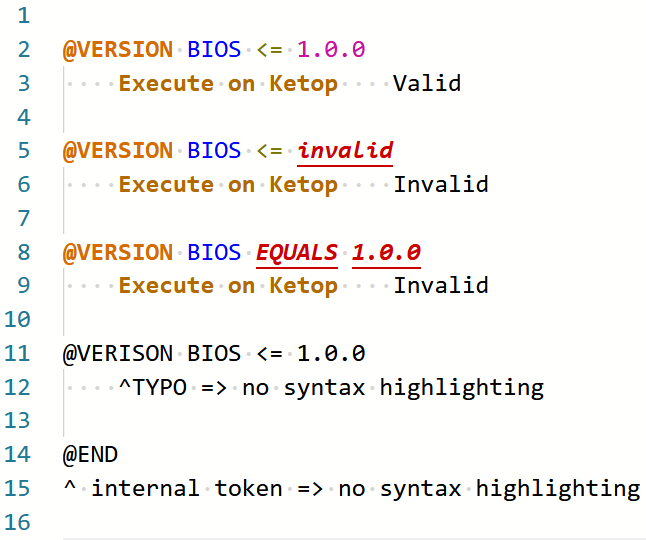
\includegraphics[width=0.75\linewidth]{pics/SyntaxHighlighting/SyntaxWHITE.png}
    \captionsetup{justification=centering,singlelinecheck=false}
    \caption{
      Syntax Highlighting in Action\\
{\small\itshape (color scheme was modified for better visibility in print)}}    
    \label{fig:syntax_highlighting}
\end{figure}

\section{Monaco Editor Setup}

The frontend application already used the Monaco Editor to provide basic syntax highlighting for standard Robot Framework scripts with the Monarch library \cite{MonacoGithub, MonacoMonarchDocs}.
Monaco is the underlying technology of Visual Studio Code and can be used in frontends through packages. The package that was used was outdated and a few other architectural issues had to be fixed, before the syntax highlighting could be implemented.

\subsection{Legacy Version Conflicts}

Over time the frontend ecosystem of the project has been updated to Angular 15, but the existing editor integration was still based on the widely used wrapper library \texttt{ngx-monaco-editor}. Unfortunately, this specific package was no longer being updated.  It officially only supported Angular up to version 12 \cite{DeprecatedNgxMonaco}. Previously developers used the npm force flag during installation to make the project compile using this already deprecated package, bypassing the dependency conflicts.

This workaround made it possible for the legacy code to somehow continue working, but it also created major risks for maintainability and the build process. Forcing npm installation is a bad practice since it only covers up package mismatches and other errors. Because of this, there is a major risk that one might get unpredictable runtime behaviors \cite{npmForceDocs}. Since we do not want that, especially later on in production, the package needed to be replaced.

After some research, the best and most widely used package, fitting exactly our requirements, seemed to be \texttt{ngx-monaco-editor-v2}. This version is an actively maintained community fork that is compatible with mordern Angular versions \cite{NgxMonacoEditorV2}.

The migration was handled in several steps to ensure a stable base. The \texttt{package.json} had to be updated, then the \texttt{app.module.ts} was refactored to match the new library and finally the asset paths in \texttt{angular.json} had to be updated.

\subsection{Custom Theme}

A custom Monaco theme was required to map the custom syntax to the correct colors. The requirement for that theme, was for the colors to stand out compared to the standard Robot Framework syntax.

The editor worked fine with its predefined default designs, but as soon as a newly created custom design was applied, a runtime error occurred: \texttt{Uncaught TypeError: this.themeData.colors is undefined}. This error completely stopped the editor from rendering any custom syntax highlighting.

Looking in the documentation gave me a hint in the right direction. The engine of Monaco is rather strict, so a \texttt{colors} object has to be provided for a theme, even if it is empty and never used \cite{MonacoThemeColorsAPI}. 

The solution was to add an empty \texttt{colors} object to the theme definition. Listing \ref{lst:theme_definition} shows the working theme configuration, which includes the required \texttt{colors} property alongside the specific token rules.

\begin{lstlisting}[caption={Custom monaco theme including the required color object}, label={lst:theme_definition}, float=htbp]
// Definition of the custom language theme
(<any>window).monaco.editor.defineTheme('robot-theme', {
  base: 'vs-dark',
  inherit: true,
  rules: [
    { token: 'variables', foreground: '#9CDCFE' },
    { token: 'keywords', foreground: '#ffe18f', fontStyle: 'bold' },
    { token: 'modifier', foreground: '#f09c00', fontStyle: 'bold' },
    { token: 'invalid', foreground: '#ff0000', fontStyle: 'underline italic' },
    // [...]
  ],
  colors: {} // Required to prevent 'this.themeData.colors is undefined'
});
\end{lstlisting}

\section{Monarch Lexer for Custom Annotations}

After the editor and theme were successfully configured, the core task was to define the syntax rules for the custom grammar of the Script Assembler. The already in use Monaco Editor uses Monarch for syntax highlighting, which works declaratively. Developers define lexers using JSON configuration objects instead of writing complex parser code \cite{MonacoMonarchDocs}.

\subsection{Tokenization and State Machine}

Monarch basically just uses Regex to handle the tokenization. The step-by-step-process starts with the lexer, that reads the document text in order and tries  to match the defined regular expression patterns. When it finds a match, the matched text is assigned a specific token class. This can be a specific keyword or a comment or it could also just be a newly defined custom modifier. The editor then maps these token classes to the specific color values defined in the active theme.

A global list of Regex rules is sufficient for simple languages. But for the custom annotations there is a need for context-aware parsing. For example, the arguments that follow an \texttt{@VERSION} annotation should be highlighted, but if the same argument is written in a comment it should not.

Monarch's state machine solved this problem. The lexer starts in a default \texttt{@root} state, when a specific pattern is matched, the lexer jumps into a different, explicitly defined state, and different Regex rules apply in this new state.

\subsection{Handling Modifiers and Arguments}

The annotations can be roughly divided into two categories. Those without any arguments and those with specific argument structures.

Modifiers without arguments, such as \texttt{@BRACKETSTART}, are simple to implement. As shown in Listing \ref{lst:root_tokenizer}, when the lexer encounters this keyword, it transitions to an \texttt{@endOfLine} state. This state  makes sure that no more text is accepted on this line. 

\begin{lstlisting}[caption={Monarch tokenizers root state}, label={lst:root_tokenizer}, float=htbp]
tokenizer: {
  root: [
    // Standard Robot Framework variables
    [/[\$@]\{[\w_/]+\}/, 'variables'],

    //#region MODIFIERS
    [/@(?:PREAMBLE)\b/, 'modifier', '@preambleArg'],
    // Modifiers without any arguments transition to @endOfLine
    [/@(?:BRACKETSTART|BRACKETEND)\b/, 'modifier', '@endOfLine'], 
    // Modifiers with complex arguments transition to their specific states
    [/@(?:VERSION)\b/, 'modifier', '@versionArgsIdentifier'],
    [/@(?:OS)\b/, 'modifier', '@osArg'],
    //#endregion
    
    // [...]
  ],
// ...
\end{lstlisting}

Modifiers with arguments are more difficult, because hey require a more complex sequence of state transitions. The modifier \texttt{@VERSION} is a good example of this as the version check needs three different components. Also important is,  they have to be in an exact order, starting with an identifier (the BIOS or software name), than a comparison operator (e.g., <, >=), and at last a valid semantic version string.

A chain of states was implemented, Root to identifier, Identifier to operator, Operator to version. That means that when \texttt{@VERSION} is found in the \texttt{@root} state, the lexer transitions to \texttt{versionArgsIdentifier}. Once a valid word is found there, it transitions to \texttt{versionArgsOperator} and finally to \texttt{versionArgsSemver}.

This ``state machine'' approach guarantees that the syntax highlighting exactly fits to the strict sequence that the parser needs. Listing \ref{lst:version_states} shows this state chain in detail. 

\begin{lstlisting}[caption={State transitions for the \texttt{@VERSION} modifier}, label={lst:version_states}, 
  breaklines=true, breakatwhitespace=false, float=htbp ]
versionArgsIdentifier: [ 
  // Entry point: match a word, then proceed to operator state
  [/[\w_]+/, 'arg.word', '@versionArgsOperator'],
  [/\n/, 'invalid', '@root'],
  [/./, 'invalid']
],
versionArgsOperator: [
  // Match comparison operators, then proceed to semantic version state
  [/(?:[<>]=?)|(?:[!=]=)/, 'arg.operator', '@versionArgsSemver'],
  [/\n/, 'invalid', '@root'],
  [/./, 'invalid']
],
versionArgsSemver: [
  // Match standard semantic versioning format
  // https://semver.org/#is-there-a-suggested-regular-expression-regex-to-check-a-semver-string
  [/(0|[1-9]\d*)\.(0|[1-9]\d*)\.(0|[1-9]\d*)(?:-((?:0|[1-9]\d*|\d*[a-zA-Z-][0-9a-zA-Z-]*)(?:\.(?:0|[1-9]\d*|\d*[a-zA-Z-][0-9a-zA-Z-]*))*))?(?:\+([0-9a-zA-Z-]+(?:\.[0-9a-zA-Z-]+)*))?/, 'arg.version'],
  [/\n/, '', '@root'],
  [/./, 'invalid']
],
\end{lstlisting}

The Regex for the semantic version argument might look complicated and hard to maintain, but it is the officially provided Regex by the organization behind semantic versions. 

\section{Troubleshooting and Error Handling}

After solving the correct highlighting of valid syntax, the next tasks were to handle edge cases and wrong inputs. 

During the implementation of the lexer, two main problems appeared, firstly to prevent ``state bleed'' over multiple lines,  secondly to provide visual error feedback without using a dedicated Language Server.

\subsection{Fixing State Bleed}

The custom EBNF grammar for the Script Assembler is strictly line-bound, so an annotation has to be strictly on a singular line. So if a line break occurs the editor should return to the standard context used for the syntax highlighting of the Robot Framework.

In the beginning, this caused a big conflict with Monarch's stateful tokenization. When the lexer goes into a state like \texttt{versionArgsIdentifier}, it just stays inside it until an explicit command such as \texttt{@root} or \texttt{@pop} is triggered. If a developer typed the keyword \texttt{@VERSION} and then pressed the Enter key without any arguments, the lexer got stuck in the \texttt{versionArgsIdentifier} state on the next line. Because of this, normal Robot Framework code on the following lines was wrongly checked against the version argument regular expressions. This completely destroyed the syntax highlighting for the whole rest of the file (see Figure \ref{fig:statebleed} for example).

\begin{figure}[hbtp]
    \centering
    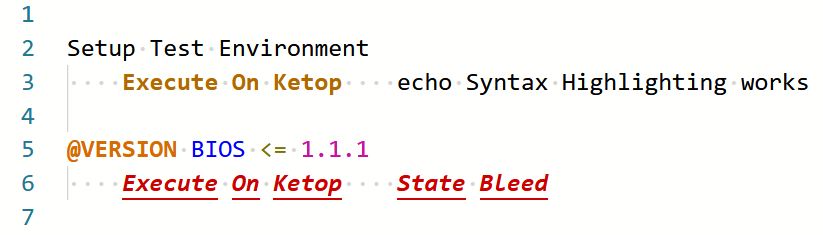
\includegraphics[width=1\linewidth]{pics/SyntaxHighlighting/state-bleed-white.png}
    \caption{State bleed in the editor when line breaks are not included}
    \label{fig:statebleed}
\end{figure}


To fix this ``state bleed'', the lexer had to recognize line breaks as termination triggers. Normally, Monarch works line-by-line and does not pass line break characters to the Regex engine. To change this, the \texttt{includeLF} property was enabled in the language configuration (see Listing \ref{lst:monarch_config_lf}).

\begin{lstlisting}[caption={\texttt{includeLF} in the Monarch config}, label={lst:monarch_config_lf}, float=htbp]
(<any>window).monaco.languages.setMonarchTokensProvider('robot', {
  ignoreCase: true,
  includeLF: true, // Exposes newline to the regex engine
  tokenizer: {
    // tokenizer rules ...
  }
});
\end{lstlisting}

With \texttt{includeLF} set to true, line breaks can be recognized. As can be seen in the state machine definition in Listing \ref{lst:version_states}, each argument state received a new rule for handling the newline character: \texttt{[/\textbackslash n/, 'invalid', '@root']}. Sometimes the lexer just resets to the \texttt{@root} state without marking an error. This is used when a line break is allowed and does not count as a syntax mistake in that specific case. This ensures that a line break always returns the lexer to the \texttt{@root} state and so protects the highlighting of all following code.

\subsection{Visualizing Syntax Errors}

A major goal for the fronted-editor was to show syntax errors to the user right away, but there was a strict rule for this. The error highlighting had to work only through the Monarch configuration, because a complex language server or an extra linter were not an option, as tools like that just use too many resources.

This was quite a problem because Monarch is really just a lexical analyzer, meaning a lexer, and not a semantic parser \cite{MonacoMonarchDocs};~\cite[pp.~5-8]{Aho2006}. It only uses regular expressions to map strings to token classes. It does not know anything about ``errors'' or ``warnings''. It also cannot draw the typical red wavy lines, that are used for code defects in modern \glspl{ide}.

To solve this problem, a visual workaround had to be built with a custom token class called \texttt{invalid}. In the custom Monaco Theme (see Listing \ref{lst:theme_definition}), this category got a unique style with red text-color,  italic style and an underline.

This \texttt{invalid} category then served as a catch-all mechanism in the state machine. Monarch always checks the rules of a state from top to bottom \cite{MonacoMonarchDocs}. By placing the rule \texttt{[/./, 'invalid']} at the very end of a states rule list, any character that does not match the expected valid patterns or the newline reset automatically falls through to this fallback rule.

A good  example for this is the modifier \texttt{@BRACKETSTART}. As it does not allow any arguments, the following happens by running the system. When the lexer sees this exact keyword, it switches to the \texttt{endOfLine} state (see Listing \ref{lst:end_of_line_state}).

\begin{lstlisting}[caption={The \texttt{endOfLine} state}, label={lst:end_of_line_state}, float=htbp]
endOfLine: [
  [/\n/, '', '@root'], // Valid: line ends, return to root
  [/./, 'invalid']     // Error: any other character is invalid
],
\end{lstlisting}

For example for the case, when a developer accidentally types a  \texttt{@BRACKETSTART argument}, the lexer first recognizes the annotation, jumps to the \texttt{endOfLine} state. There, it expects the end of the line. Instead, it encounters a space, and the word ``argument''. Because these characters do not match the \texttt{/\textbackslash n/} Regex, they fall through to the \texttt{/./} rule. As a result, the string ``argument'' turns red, gets underlined and italic, and by doing so, shows the developer a syntax error. The user sees a clear syntax error right away without backend validation. Real-time error feedback is a useful feature, and even better, everything remains strictly within the boundaries of the Monarch lexer architecture.

\section{Limitations}

Being able to catch errors early with the syntax highlighting was definitely worth the addition. But even with all the effort, there is a limitation that could not be fixed, since there is a conflict between the rules of the two used languages, which could only be fixed through a custom Language Server.

The EBNF grammar for the backend is strictly case-sensitive. That means, all annotations and modifiers like \texttt{@VERSION} or \texttt{@OS}, have to be in uppercase, and different spelling leads to  a syntax error during transpilation.

The standard Robot Framework language on the other hand works differently. Here upper and lower case do not matter, the language is case-insensitive \cite{RobotFrameworkCaseInsensitive}. Because of this, the \texttt{ignoreCase} property of the Monarch lexer must be set to true globally, if not, the normal keywords and variables do not get the correct highlighting (see example in Figure \ref{fig:case-sensitivity-issue}). 

\begin{figure}[htb]
    \centering
    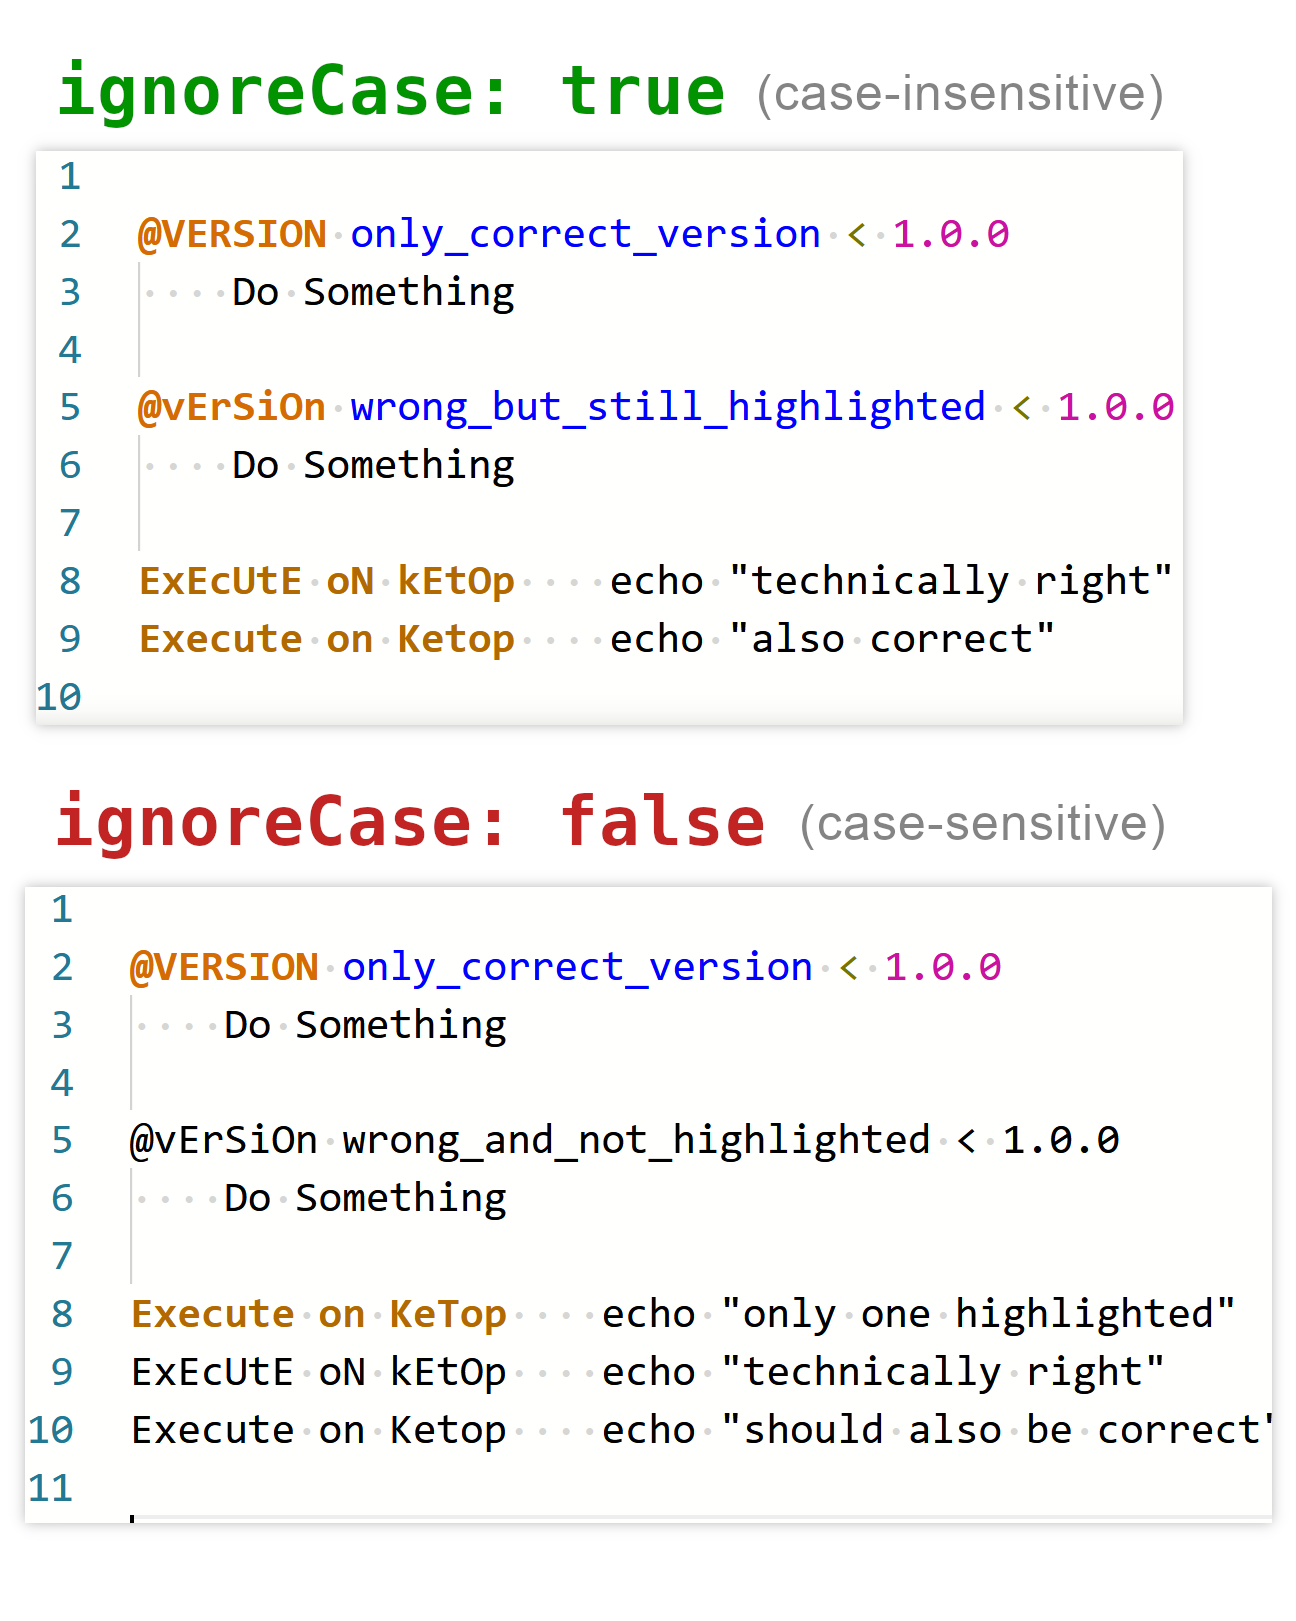
\includegraphics[width=0.8\linewidth]{pics/SyntaxHighlighting/case-sensitivity-issue.png}
    \caption{Case sensitivity issues in syntax highlighting}
    \label{fig:case-sensitivity-issue}
\end{figure}


The Monarch API only allows this setting for the entire language, because it is only possible through the global \texttt{ignoreCase} property defined in the \texttt{IMonarchLanguage} interface. A custom override for one tokenizer rule(\texttt{IMonarchLanguageRule}) or a single state is not possible. Therefore, the setting affects everything, the entire tokenizer. In the implemented editor configuration this global setting also affects the custom annotation rules, and as a result, if a developer types \texttt{@version} in lowercase, the frontend lexer still matches the rule and applies the corresponding syntax highlighting. But with the same script, the validation crashes when the backend EBNF parser takes the script. The reason is that the parser strictly needs the uppercase syntax \cite{MonacoMonarchTypes0341}.

This limitation leads to a small difference between the visual representation and the backend, but it is an unavoidable compromise. Disabling \texttt{ignoreCase} globally completely breaks the standard Robot Framework code highlighting, and that code is the vast majority of the file. That is why it is more important, that the base language simply has to function. This was the basis for the final architectural decision together with KEBA, even if it means the developer will only notice the error during transpilation and not while typing.

